\section{Preparação dos dados}
\label{sec:metodos-preparacao-dataset}

% RESAMPLING DO DATASET -------------------------------------------

Conforme introduzido na seção anterior, o número de amostras disponíveis por sinal não está balanceado homogeneamente no ASL-Phono e, como consequência, isso poderia influenciar de maneira indesejada o desempenho dos modelos utilizados nos experimentos adiante, fazendo com que algumas classes fossem extremamente favorecidas e, outras, severamente penalizadas.

% Conforme observa-se pela \autoref{tab:dataset-phono-stats}, o ASL-Phono apresenta um desbalanceamento no número de amostras disponíveis por sinal. Em média, há 3,68 amostras disponíveis por sinal porém, enquanto alguns sinais têm apenas 1 amostra, outros apresentam um número atípico de 59. Isso poderia influenciar o desempenho dos modelos utilizados adiante, uma vez que durante o treinamento alguns sinais seriam favorecidos e, outros, penalizados. 

Devido a isso, serão aplicados dois procedimentos para tentar equalizar essa proporção. Primeiro, serão descartados aqueles sinais que apresentam apenas 1 amostra disponível, uma vez que esse número é insuficiente para permitir o modelo aprender e generalizar tais sinais, sobretudo porque o \textit{dataset} será particionado em mais de um subconjunto durante seu treinamento e todas as classes precisam estar igualmente representadas neles.

Em seguida, será realizada uma reamostragem do \textit{dataset} com o intuito de balancear melhor a proporção de amostras.
Será utilizado para isso uma reamostragem \textit{Naive Random Under-Sampling} (ou sub-amostragem aleatória ingênua), que reduz o número de amostras super-representadas selecionando aleatoriamente algumas delas e, em seguida, uma \textit{Naive Random Over-Sampling} (ou sobre-amostragem aleatória ingênua) que, por sua vez, aumenta o número de amostras sub-representadas replicando aleatoriamente algumas existentes \cite{he-2013-imbalanced}.

A \autoref{eqn:resampling-target} define a operação aplicada para definir o número de amostras \(n'\) a ser obtido para cada sinal por processo de reamostragem. Nela, \(\overline{m}\) refere-se à média de amostras por sinal e \(n\) é o número atual de amostras para aquele sinal:

\begin{equation}
    \label{eqn:resampling-target}
    n' = round( \overline{m} + \ln(n) )
\end{equation}

% Onde \(\overline{m}\) refere-se ao número médio de amostras por sinal no \textit{dataset} e \(n\) é o número de amostras para aquele sinal. 

Observe na \autoref{fig:dataset-resampling-depois} a nova distribuição das amostras no \textit{dataset}. De uma forma resumida, ao comparar com a \autoref{fig:dataset-resampling-antes}, percebe-se que a reamostragem homogeneizou a relação de amostras por sinal em torno da nova média do conjunto, trazendo para essa região também os antigos \textit{outliers} (valores atípicos ou pontos fora da curva).

% Observe na \autoref{subfig:dataset-resampling-antes} um perfil detalhado dos dados antes da reamostragem. É possível perceber que o número de amostras é bastante disperso pelo eixo horizontal do gráfico: por exemplo, 726 sinais apresentam 2 amostras disponíveis; seguidos por 552 sinais com 4 amostras; mas, no outro extremo, temos que apenas um número muito pequeno de sinais (entre 1 e 3) apresentam um grande número de amostras disponíveis (entre 13 e 59), respectivamente.

\figura
{fig:dataset-resampling-depois} % Label
{capitulos/metodos/imagens/dataset_resampling_depois} % Path
{height=5.5cm} % Size
{Distribuição do número de amostras por sinal após a reamostragem} % Caption
{} % Citation


% \begin{figure}[ht!]
%     \centering
%     \caption{
%         \textmd{Número de amostras disponíveis por sinal (\subref{subfig:dataset-resampling-antes}) antes da reamostragem e (\subref{subfig:dataset-resampling-depois}) após a reamostragem do ASL-Phono. Por exemplo, lê-se que 726 sinais possuem 2 amostras disponíveis antes da reamostragem.}
%     }
%     \subcaptionbox{\label{subfig:dataset-resampling-antes}}{
%         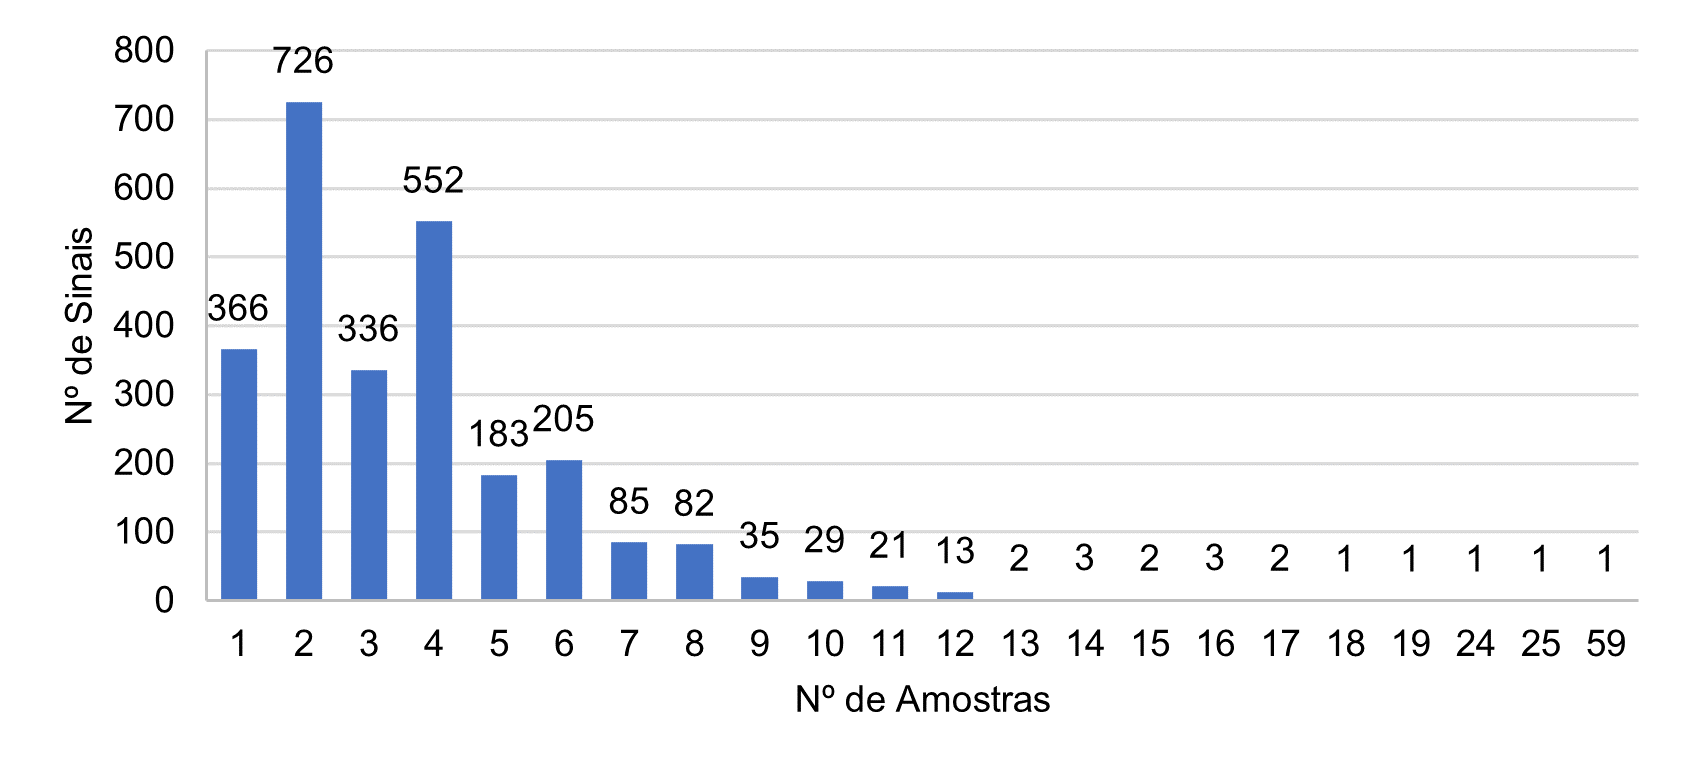
\includegraphics[height=6cm]{capitulos/metodos/imagens/dataset_resampling_antes}
%     }%
%     \hspace{1cm}
%     \subcaptionbox{\label{subfig:dataset-resampling-depois}}{
%         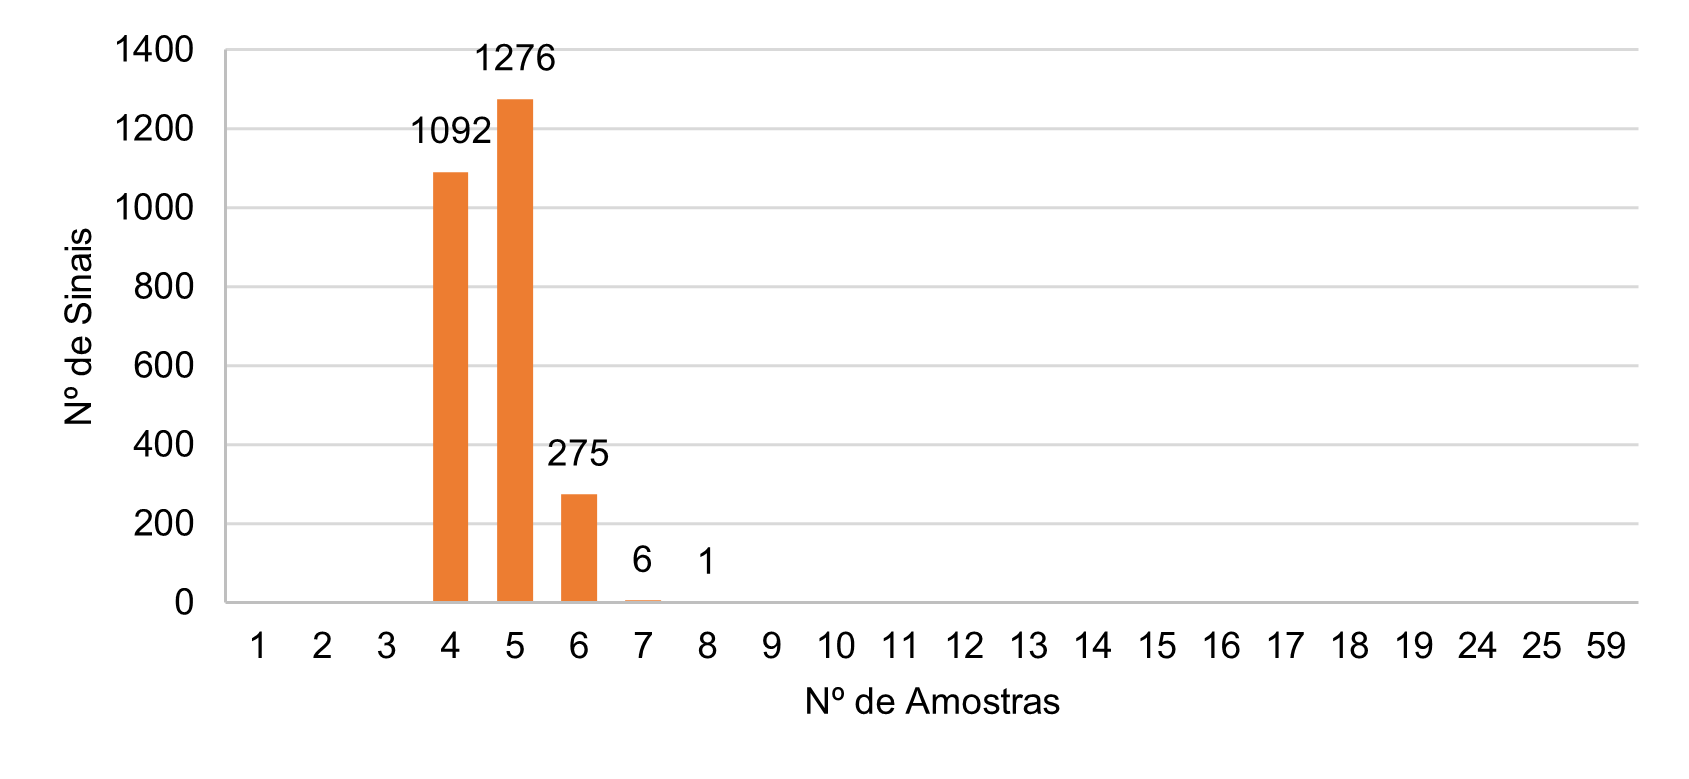
\includegraphics[height=6cm]{capitulos/metodos/imagens/dataset_resampling_depois}
%     }%
%     \nomefonte{}
%     \label{fig:dataset-resampling}
% \end{figure}



% COMPACTAÇÃO DAS FEATURES -------------------------------------------

Por fim, será aplicada uma transformação às amostras do ASL-Phono para tornar a estrutura apresentada no \autoref{cod:sample-json-phono} compatível com a entrada dos modelos que serão aplicados mais adiante.
Para isso, serão compactados os valores informados para os atributos fonológicos de cada \textit{frame} em uma ``palavra'' única, fazendo com que a sequência de \textit{frames} seja então representada como uma sequência dessas palavras.

Por exemplo, considerando-se um \textit{frame} contendo dois atributos com os valores ``\textit{valor\_atributo\_1}'' e ``\textit{valor\_atributo\_2}'', ao compactá-los, eles primeiro seriam abreviados para ``\textit{va1}'' e ``\textit{va2}'' e, em seguida, concatenados para formar uma palavra ``\textit{va1-va2}''.  A sequência de \textit{frames} da amostra tornaria-se, portanto, algo semelhante a uma sequência de palavras \textit{\{``va1-va2'', ``va3-va4'', \dots, ``vaN-vaN''\}}.

Observe na \autoref{tab:codificacao-bloco} um exemplo mais próximo do contexto real para esse processo. Na primeira linha estão os valores originais dos atributos do \textit{frame}; na segunda, os valores abreviados; e, na terceira, a palavra formada através da concatenação deles.

% Para tornar as amostras do ASL-Phono compatíveis com a entrada dos modelos que serão utilizados mais adiante, aplicamos uma transformação simples que consiste em codificar seus atributos fonológicos como blocos ou ``palavras'' únicas, mais compactas. Ou seja, ao invés de utilizar como entrada sequências de frames que contêm propriedades aninhadas, adotamos aqui sequências de blocos compactos que codificam a mesma informação de uma forma mais amigável a modelos sequenciais.

% Observe na \autoref{tab:codificacao-bloco} um exemplo deste processo. Na primeira linha, temos os valores originais das propriedades providas para o frame de uma amostra do ASL-Phono; na segunda linha, geram-se acrônimos a partir desses atributos para realizar uma primeira compactação -- mas que não é um passo necessariamente obrigatório; na terceira linha, temos um bloco ou palavra única gerada pela composição desses acrônimos; finalmente, na última linha, temos o exemplo de uma sequência desses blocos.

% Please add the following required packages to your document preamble:
% \usepackage{graphicx}
% \usepackage[table,xcdraw]{xcolor}
% If you use beamer only pass "xcolor=table" option, i.e. \documentclass[xcolor=table]{beamer}
\begin{table}[ht!]
    \centering
    \caption{Exemplo de compactação dos atributos fonológicos do \textit{frame} de uma amostra do ASL-Phono em uma ``palavra''}
    \label{tab:codificacao-bloco}
    \resizebox{0.95\textwidth}{!}{%
        \begin{tabular}{r|cccccc}
            \hline
            \rowcolor[HTML]{EFEFEF}
            \multicolumn{1}{l|}{\cellcolor[HTML]{EFEFEF}} & \multicolumn{6}{c}{\cellcolor[HTML]{EFEFEF}Atributos}                                                                                                                                                                                                                          \\ \cline{2-7}
            \rowcolor[HTML]{EFEFEF}
                                                          & \multicolumn{3}{c|}{\cellcolor[HTML]{EFEFEF}Mão dominante}                    & \multicolumn{3}{c}{\cellcolor[HTML]{EFEFEF}Mão não-dominante}                                                                                                                                  \\
            \rowcolor[HTML]{EFEFEF}
                                                          & Movimento                                                                     & Orientação                                                    & \multicolumn{1}{c|}{\cellcolor[HTML]{EFEFEF}Config. mão} & Movimento                  & Orientação           & Config. mão     \\ \hline
            Valores originais                             & \textit{right\_up}                                                            & \textit{left}                                                 & \multicolumn{1}{c|}{\textit{bentBL}}                     & \textit{left\_front\_down} & \textit{back\_right} & \textit{bentBL} \\
            Valores abreviados                            & \textit{ru}                                                                   & \textit{l}                                                    & \multicolumn{1}{c|}{\textit{bentBL}}                     & \textit{lfd}               & \textit{br}          & \textit{bentBL} \\ \hline
            {\color[HTML]{3531FF} Palavra}                & \multicolumn{6}{c}{{\color[HTML]{3531FF} \textit{ru-l-bentBL-lfd-br-bentBL}}}                                                                                                                                                                                                  \\ \hline
        \end{tabular}%
    }
    \nomefonte{}
\end{table}
